\documentclass[a4paper, 14pt]{extarticle}

\usepackage{../../latexDependencies/misc/preamble}

\geometry{a4paper}

\raggedright  % Add this line after the preamble

\begin{document}

\newgeometry{left=25mm, right=25mm, top=20mm, bottom=20mm}

\graphicspath{ {images} } 

% Customize section, subsection, subsubsection and paragraph styles
\titleformat{\section}
  {\normalfont\large\bfseries}{\thesection}{1em}{}

\titleformat{\subsection}
  {\normalfont\normalsize\bfseries}{\thesubsection}{1em}{}

\titleformat{\subsubsection}
  {\normalfont\small\bfseries}{\thesubsubsection}{1em}{}

\titleformat{\paragraph}
  {\small\small\bfseries}{\theparagraph}{1em}{}

\setcounter{tocdepth}{5}
\setcounter{secnumdepth}{5}

\pagenumbering{roman}

\tableofcontents\newpage

\pagenumbering{arabic}
\setcounter{page}{1}

\setstretch{1}
\linespread{1.1}

\setlength{\parindent}{0pt}

\fontsize{12pt}{16pt}\selectfont

\definecolor{myblue}{HTML}{0A88C2}
\definecolor{myred}{HTML}{FF1B1C}
\definecolor{mygreen}{HTML}{386641}

\lstdefinestyle{mystyle}{
    basicstyle=\ttfamily\footnotesize,
    keywordstyle=\color{myblue},
    stringstyle=\color{myred},
    commentstyle=\color{green!50!black},
    showstringspaces=false,
    frame=leftline, 
    framesep=10pt, 
}

% Set the style for Python code
\lstset{style=mystyle, extendedchars=\true}

% --------------------------------------START--------------------------------------

\section*{Задание}\vspace{-20pt}\rule{\linewidth}{0.1mm}
\addcontentsline{toc}{section}{\protect\numberline{}Задание}

Для унимодальной на отрезке $[e; f]$ функции $f(x) = a x^3 + b x^2 + c x + d$ найти минимум с использованием 
следующих методов одномерной оптимизации.
Использовать методы:
\begin{itemize}
    \item \textbf{Метод 1:} Метод равномерного поиска \\
    \item \textbf{Метод 2:} Метод ломаных \\
    \item \textbf{Метод 3:} Метод секущих \\
    \item \textbf{Метод 4:} Метод Ньютона \\
\end{itemize}

Построить математическую модель задачи, решить ее аналитически.
Разработать программу одномерной минимизации на Python с использованием
библиотек Numpy, Scipy, Matplotlib и убедиться в правильности результата,
сравнив его с аналитическим решением.

\section*{Алгоритм}\vspace{-20pt}\rule{\linewidth}{0.1mm}
\addcontentsline{toc}{section}{\protect\numberline{}Алгоритм}

\begin{enumerate}
    \item Выбрать самостоятельно и описать исходную функцию, привести примеры задач, в которых могут возникнуть подобные исходные данные. Привести примеры задач, которые решаются с использованием одномерной оптимизации. Описать теоретически используемые методы решения задачи.

    \item Проанализировать исходные данные. Проверить уникальность функции. Изобразить исходную функцию при помощи библиотеки matplotlib, привести код. Сделать предположения о минимуме.

    \item Решить задачу аналитически. Описать нахождение минимума каждым методом вручную. Изобразить результаты графически при помощи библиотеки matplotlib, привести код для построения значений. (Аналитическое решение можно выполнить от руки, приложить в отчет отсканированные фото)

    \item Решить задачу на языке python с использованием библиотеки питона, привести код, привести результат решения. Полученный результат изобразить графически при помощи библиотеки matplotlib, привести код для построения значений.

    \item Решить задачу на языке python с использованием библиотеки scipy и matplotlib. Полученный результат изобразить графически при помощи библиотеки matplotlib, привести код для построения значений.

    \item Сравнить решения, полученные вручную и с помощью решения на python, построить решения графически. Оценить точность.

    \item Сделать вывод.
\end{enumerate}

\section*{Ход выполнения работы}\vspace{-20pt}\rule{\linewidth}{0.1mm}
\addcontentsline{toc}{section}{\protect\numberline{}Ход выполнения работы}
\vspace{-30pt}
\subsection*{Теоретическая справка}\vspace{-20pt}\rule{\linewidth}{0.1mm}
\addcontentsline{toc}{subsection}{\protect\numberline{}Теоретическая справка}

\textbf{\normalsize Исходная функция.}\\[0.5em]

Дана унимодальная кубическая функция $f(x) = a x^3 + b x^2 + c x + d$ на 
отрезке $[e; f]$. Унимодальность означает, что на этом отрезке функция имеет 
только один экстремум (минимум или максимум), что делает её пригодной для применения 
методов одномерной оптимизации.\\
\vspace{20pt}
\textbf{\normalsize Примеры задач, где возникают подобные исходные данные.}\\[0.5em]

\begin{itemize}
    \item \textbf{Экономика и управление}\\ 
    Оптимизация объёма производства, если затраты описываются кубической функцией 
    (например, из-за нелинейных эффектов масштаба). 
    На отрезке $[e;f]$ требуется найти объём, минимизирующий себестоимость. \\

    \item \textbf{Физика и инженерия}\\ 
    Расчёт момента времени, когда скорость движения объекта с кубической 
    зависимостью координаты от времени достигает экстремума на заданном 
    интервале $[e;f]$. \\

    \item \textbf{Биологическое моделирование}\\ 
    Поиск оптимальной концентрации вещества, при которой скорость химической 
    реакции (описываемая кубической функцией) максимальна в диапазоне $[e;f]$. \\

    \item \textbf{Материаловедение}\\ 
    Определение параметра (например, толщины материала), при котором напряжение в 
    конструкции, зависящее от параметра кубически, достигает минимального значения на 
    интервале $[e;f]$. \\
\end{itemize}
\vspace{20pt}
\textbf{\normalsize Примеры задач, решаемых одномерной оптимизацией.}\\[0.5em]

\begin{itemize}
    \item \textbf{Минимизация функции затрат}\\ 
    Найти точку $x \in [e, f]$, где функция затрат $f(x)$ достигает минимума. 
    Методы: золотое сечение, параболы. \\

    \item \textbf{Максимизация прибыли}\\ 
    Определить цену товара $x$, максимизирующую прибыль $f(x)$, 
    если зависимость прибыли от цены задана аналитически. \\

    \item \textbf{Инженерный дизайн}\\ 
    Оптимизация длины рычага в механизме для минимизации требуемого усилия, 
    где усилие выражается функцией $f(x)$. \\

    \item \textbf{Финансовый анализ}\\ 
    Поиск оптимальной доли инвестиций в актив, если доходность зависит от 
    этой доли кубически на интервале допустимых значений. \\

    \item \textbf{Научные эксперименты}\\ 
    Калибровка параметра эксперимента (например, температуры) для минимизации 
    погрешности измерений, заданной функцией $f(x)$. \\
\end{itemize}
\vspace{20pt}
\textbf{\normalsize Примечание.}\\[0.5em]

Унимодальность кубической функции на $[e;f]$ может быть обеспечена, 
даже если её производная (квадратичная функция) имеет два корня, но 
только один из них попадает в заданный отрезок. Это позволяет гарантировать 
корректность применения методов одномерной оптимизации.

\subsection*{Утилиты}\vspace{-20pt}\rule{\linewidth}{0.1mm}
\addcontentsline{toc}{subsection}{\protect\numberline{}Утилиты}

Для начала заведём вспомогательный класс для хранения данных в виде точек:

\begin{center}
    \begin{lstlisting}[language=Python]
# Define a helper class for points 
# of type (x, y)
@dataclass
class Point:
    x: float
    y: float

    def __str__(self):
        return f'(x={self.x}; y={self.y})'
    
    def __lt__(self, other):
        return self.y <= other.y
    
    def __format__(self, format_spec):
        format_x = format(self.x, format_spec)
        format_y = format(self.y, format_spec)
        return  f'(x={format_x}; y={format_y})'
    \end{lstlisting}
\end{center}

А также абстрактный класс со всеми указаными методами:

\begin{center}
    \begin{lstlisting}[language=Python]
# Define an abstract class
class Optimization(ABC):
    def __init__(self, func) -> None:
        self.func = func   

    # Метод равномерного поиска
    @abstractmethod
    def uniform_search(self, a: float, 
                             b: float,
                             n: int,
                             add_to_comparison: bool,
                             *args):
        pass

    # Метод ломаных
    @abstractmethod
    def broken_lines(self):
        pass

    # Метод секущих
    @abstractmethod
    def secant(self):
        pass

    # Метод Ньютона
    @abstractmethod
    def newton(self):
        pass
    \end{lstlisting}
\end{center}

И последний вспомогательный класс для сравнения полученных данных в дальнейшем:

\begin{center}
    \begin{lstlisting}[language=Python]
class Comparison:
    @dataclass
    class Method:
        name: str
        implementation_type: str
        result: Point
        execution_time: float
        details: str = ''

    def __init__(self) -> None:
        self.data = []

    def add_data(self, method: Method) -> None:
        self.data.append(method)
    
    def get_data(self) -> list[Method]:
        return self.data
    \end{lstlisting}
\end{center}

\subsection*{Исходные данные}\vspace{-20pt}\rule{\linewidth}{0.1mm}
\addcontentsline{toc}{subsection}{\protect\numberline{}Исходные данные}

Случайно выберем коэффициенты $a, b, c, d$ и запишем их в коде:

\begin{center}
    \begin{lstlisting}[language=Python]
# define a function
def func(x, a, b, c, d) -> float:
    return a * x**3 + b * x**2 + c * x + d

# randomly choose coefficients
A, B, C, D = 89, 45, -44, 68

INTERVAL = (-0.5, 1)

# create a Comparison object
cmpr = Comparison()
    \end{lstlisting}
\end{center}

\subsection*{Анализ данных}\vspace{-20pt}\rule{\linewidth}{0.1mm}
\addcontentsline{toc}{subsection}{\protect\numberline{}Анализ данных}

Построим график заданной функции с выбранными коэффициентами:

\begin{center}
    \begin{lstlisting}[language=Python]
myfunc = lambda x : func(x, A, B, C, D)

# create plot 
with plt.rc_context(classic_style): # use context for styles not to interfere
    fig, ax = plt.subplots(figsize=(6, 15))

    x_values = np.linspace(-1-0.25, 0.75+0.25, 100)
    y_values = myfunc(x_values)

    ax.plot(x_values, y_values, color=RICH_BLACK, linewidth=3)

    ax.set_title(f'$ f(x) = {A} \\cdot x^3 {'+' if B > 0 else ''} {B} \\cdot x^2 {'+' if C > 0 else ''} {C} \\cdot x {'+' if D > 0 else ''} {D} $')
    decorate_regular_plot(ax, '$x$', '$f(x)$')

    ax.grid(linewidth=1)

    if SAVE:
        plt.savefig(f'{IMAGES_PATH}/initial_f_plot.png', 
                    dpi=300, transparent=True)

    plt.show()
    \end{lstlisting}
\end{center}

\begin{minipage}{0.4\textwidth}
    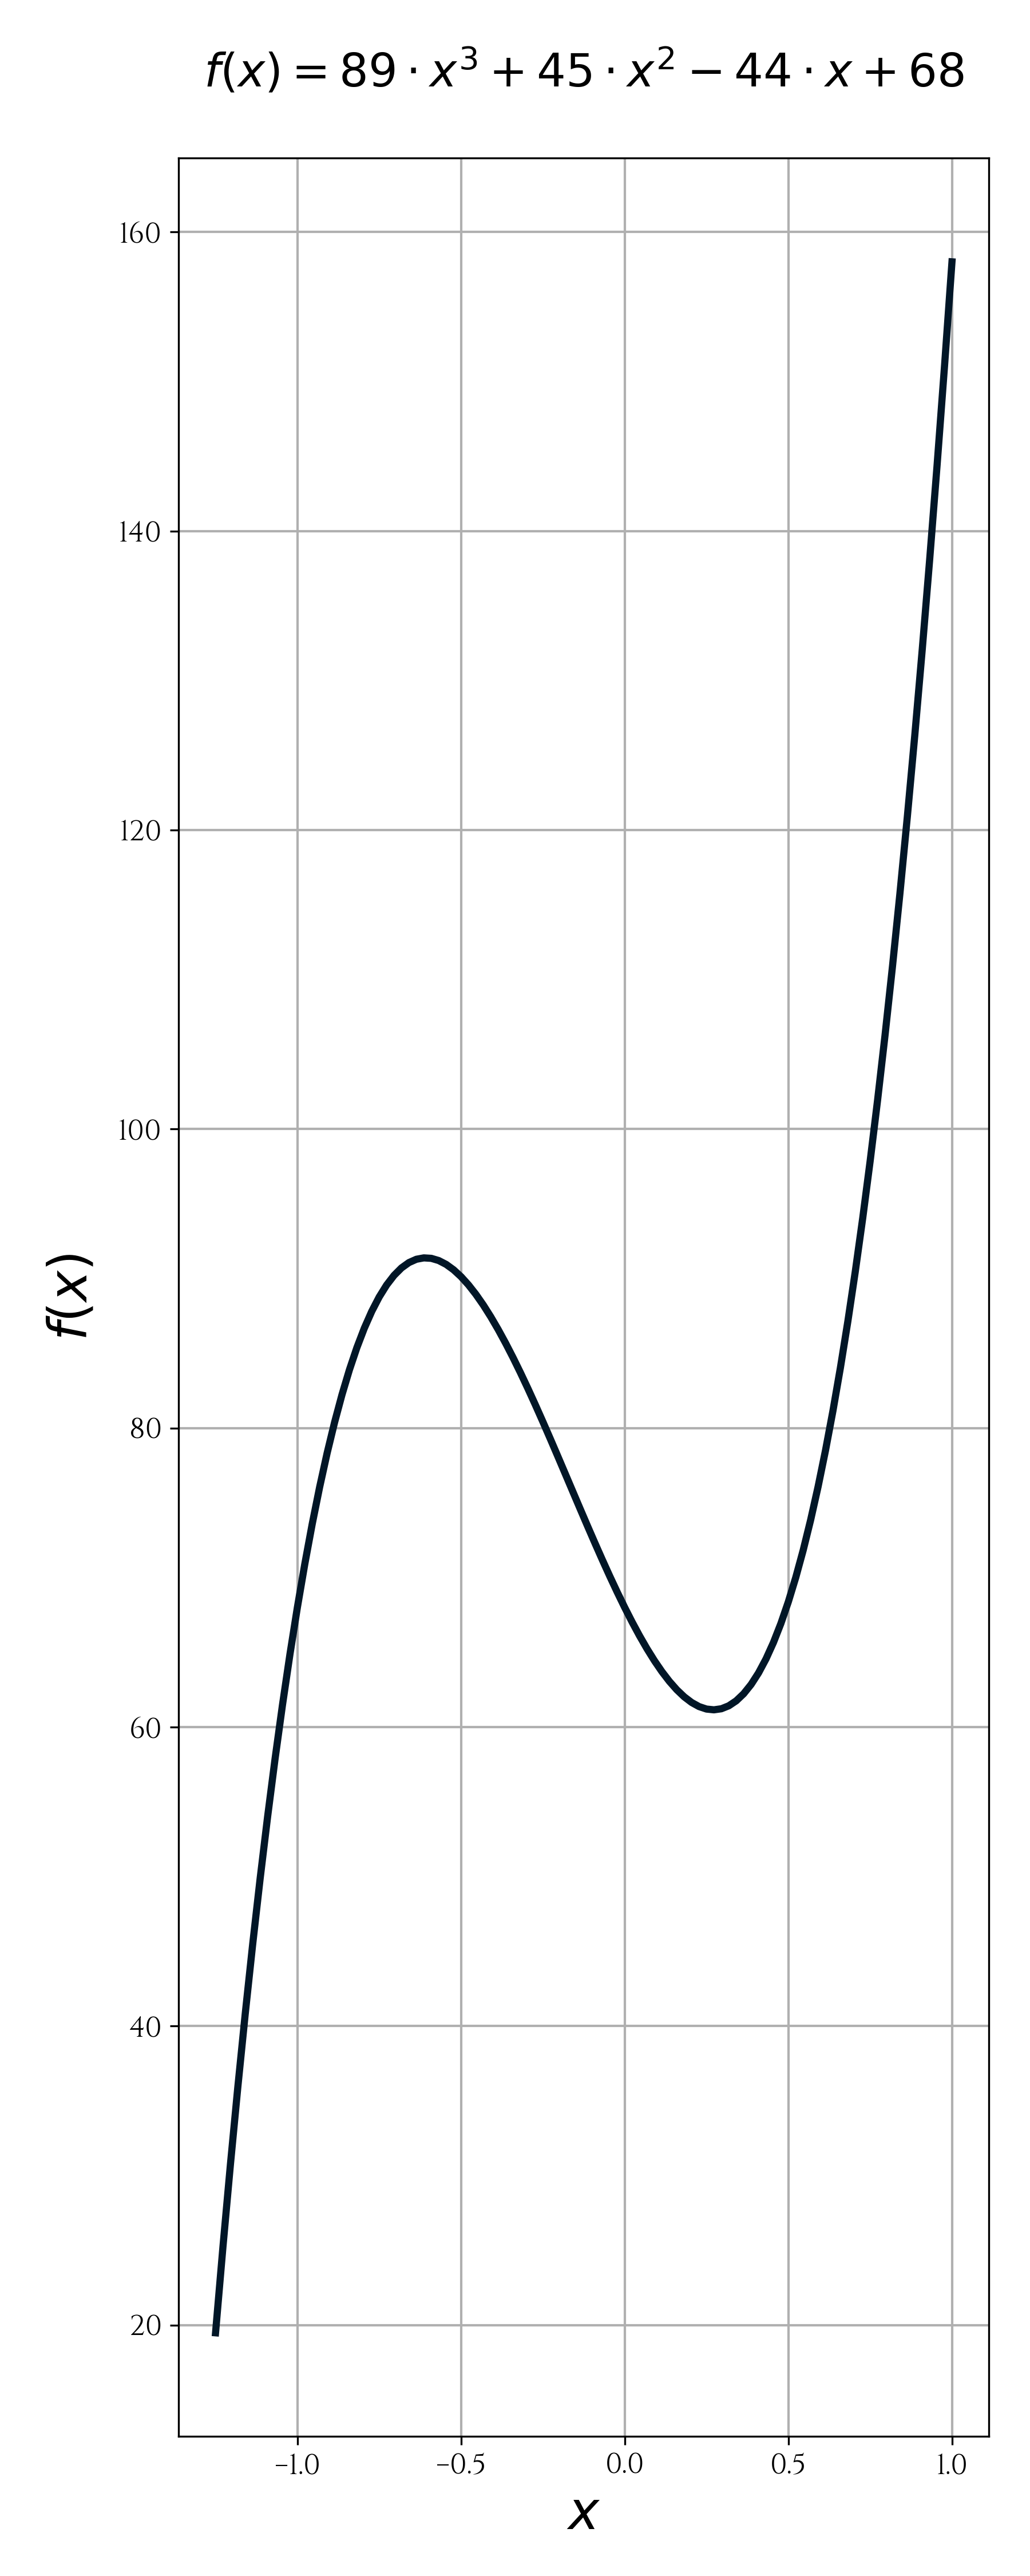
\includegraphics[width=\linewidth]{initial_f_plot}
\end{minipage}
\hfill
\begin{minipage}{0.55\textwidth}
    Как видно из графика, выбранный промежуток $([-0.5, 1])$ удовлетворяет 
    условию унимодальности. \\

    \guillemotleft На глаз\guillemotright {} можно сделать предположение, что 
    минимум находится где то в районе точки \\$x=0.3$.
\end{minipage}

% ------------------------------------------------------------------------------------
% ----------------------------------UNIFORM SEARCH------------------------------------
% ------------------------------------------------------------------------------------

\subsection*{Метод равномерного поиска}\vspace{-20pt}\rule{\linewidth}{0.1mm}
\addcontentsline{toc}{subsection}{\protect\numberline{}Метод равномерного поиска}
\vspace{-30pt}
\subsubsection*{Теория}\vspace{-20pt}\rule{\linewidth}{0.1mm}
\addcontentsline{toc}{subsubsection}{\protect\numberline{}Теория}

Метод равномерно поиска (метод перебора) - простейший из методов поиска значений 
действительно-значных функций по какому-либо из критериев сравнения 
(на максимум, на минимум, на определённую константу). Применительно к экстремальным 
задачам является примером прямого метода условной одномерной пассивной оптимизации.\\[1em]

Проиллюстрируем суть метода равномерного поиска посредством рассмотрения задачи нахождения минимума.

Пусть задана функция \( f(x): [a, b] \rightarrow \mathbb{R} \) и задача оптимизации выглядит так: \( f(x) \rightarrow \min \). Пусть также задано число наблюдений \( n \).\newpage

Тогда отрезок \([a, b]\) разбивают на \((n+1)\) равных частей точками деления:

\[
x_i = a + i \frac{(b - a)}{(n + 1)}, \quad i = 1, \ldots, n
\]

Вычисляя значения \( F(x) \) в точках \( x_i, \, i = 1, \ldots, n \), найдем путем сравнения точку \( x_m \), где \( m \) — это число от 1 до \( n \) такое, что

\[
F(x_m) = \min F(x_i) \text{ для всех } i \text{ от 1 до } n.
\]

\subsubsection*{Аналитическое решение}\vspace{-20pt}\rule{\linewidth}{0.1mm}
\addcontentsline{toc}{subsubsection}{\protect\numberline{}Аналитическое решение}

\begin{center}
    \fbox{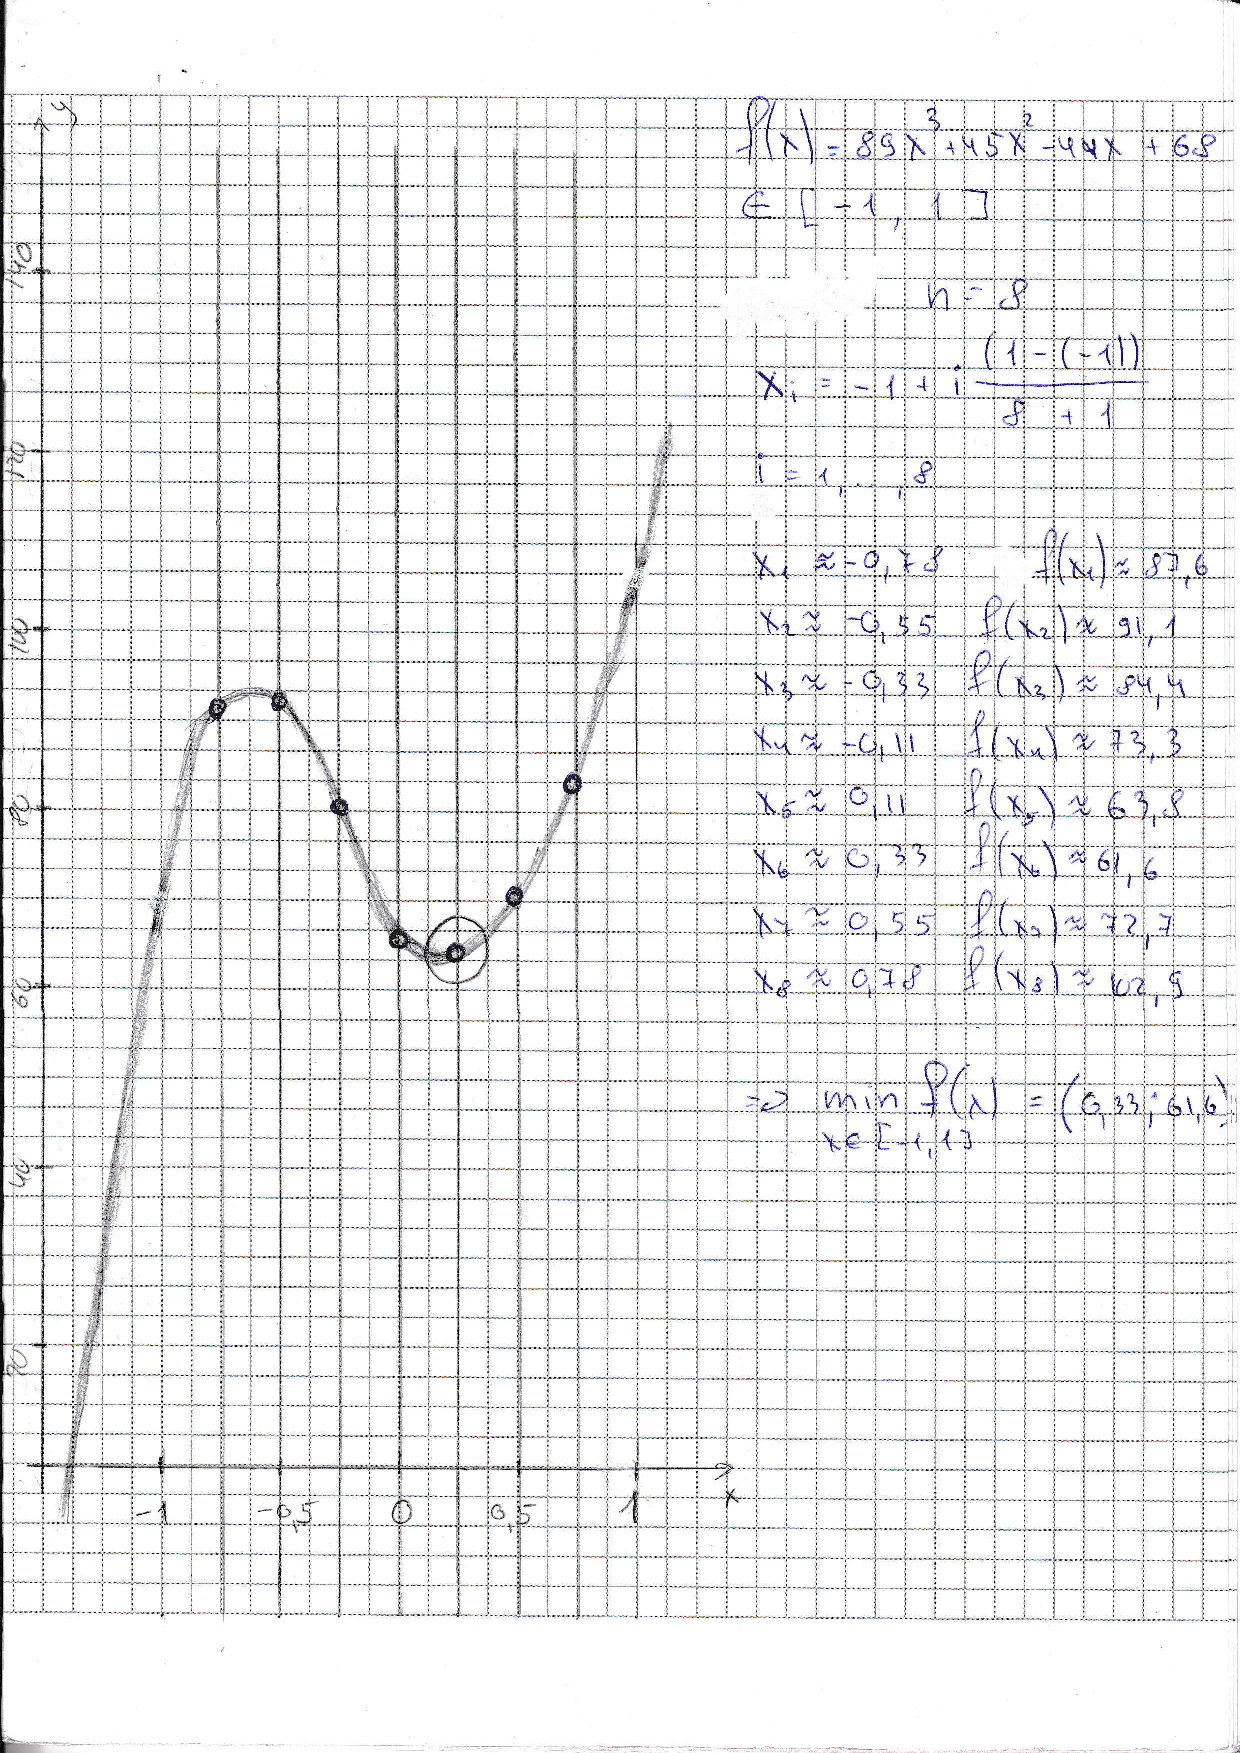
\includegraphics[width=0.8\textwidth, height=0.8\textheight, keepaspectratio]{uniform_hand.pdf}} \\
\end{center}

\subsubsection*{Реализация метода}\vspace{-20pt}\rule{\linewidth}{0.1mm}
\addcontentsline{toc}{subsubsection}{\protect\numberline{}Реализация метода}

Теперь наследуем наш ранее объявленный абстрактный класс и реализуем описанный 
метод:

\begin{center}
    \begin{lstlisting}[language=Python]
# class for analytical implementations
class OptimizationAnalytical(Optimization):
    # Метод равномерного поиска
    def uniform_search(self, a: float, 
                             b: float,
                             n: int = 1000,
                             add_to_comparison: bool = True,
                             showplot: bool = False):
        
        # start timer
        start_time = time.perf_counter()

        points, minpoint = [], None
        for i in range(1, n + 1):
            x = a + i * (b - a)/(n + 1)
            y = self.func(x)
            point = Point(x, y)
            points.append(point)

            if minpoint is None:
                minpoint = point
            else:
                minpoint = min(minpoint, point)

        # end timer
        result_time = time.perf_counter() - start_time

        # add data to Comparison class
        if add_to_comparison:
            method = Comparison.Method('uniform_search', 'analytical', 
                                        minpoint, result_time)
            cmpr.add_data(method)

        if showplot:
            # create plot 
            with plt.rc_context(classic_style): # use context for styles not to interfere
                _, ax = plt.subplots(figsize=(6, 15))

                x_values = np.linspace(-1-0.25, 0.75+0.25, 100)
                y_values = myfunc(x_values)

                # plot main function
                ax.plot(x_values, y_values, color=RICH_BLACK, linewidth=3)

                # plot vertical lines with dots
                for i, point in enumerate(points):
                    # plot lines
                    ax.axvline(x=point.x, color=RED, linestyle='--')

                    # plot dots
                    ax.scatter(point.x, point.y, color=RED, 
                               s=50, zorder=n + 1 + i + 1)

                ax.set_title(f'uniform search(n={n})')
                decorate_regular_plot(ax, '$x$', '$f(x)$')

                ax.grid(linewidth=1)

                if SAVE:
                    plt.savefig(f'{IMAGES_PATH}/uniform_search_f_plot(n={n}).png', 
                                dpi=300, transparent=True)

                plt.show()

        return [minpoint, result_time]
    \end{lstlisting}
\end{center}

И запустим на данных, разобранных вручную:

\begin{center}
    \begin{lstlisting}[language=Python]
# create optimizer and find minimum
optimizer = OptimizationAnalytical(func=myfunc)

min_point, elapsed_time = optimizer.uniform_search(*INTERVAL, showplot=True, 
                                                   n=8, add_to_comparison=False)
print(f'Minimum found at: {min_point:.6f}')
    \end{lstlisting}
\end{center}

\vfill

\begin{equation*}
    \scalebox{1.5}{
        $\downarrow$
    }
\end{equation*}

\vfill\newpage

\begin{minipage}{0.4\textwidth}
    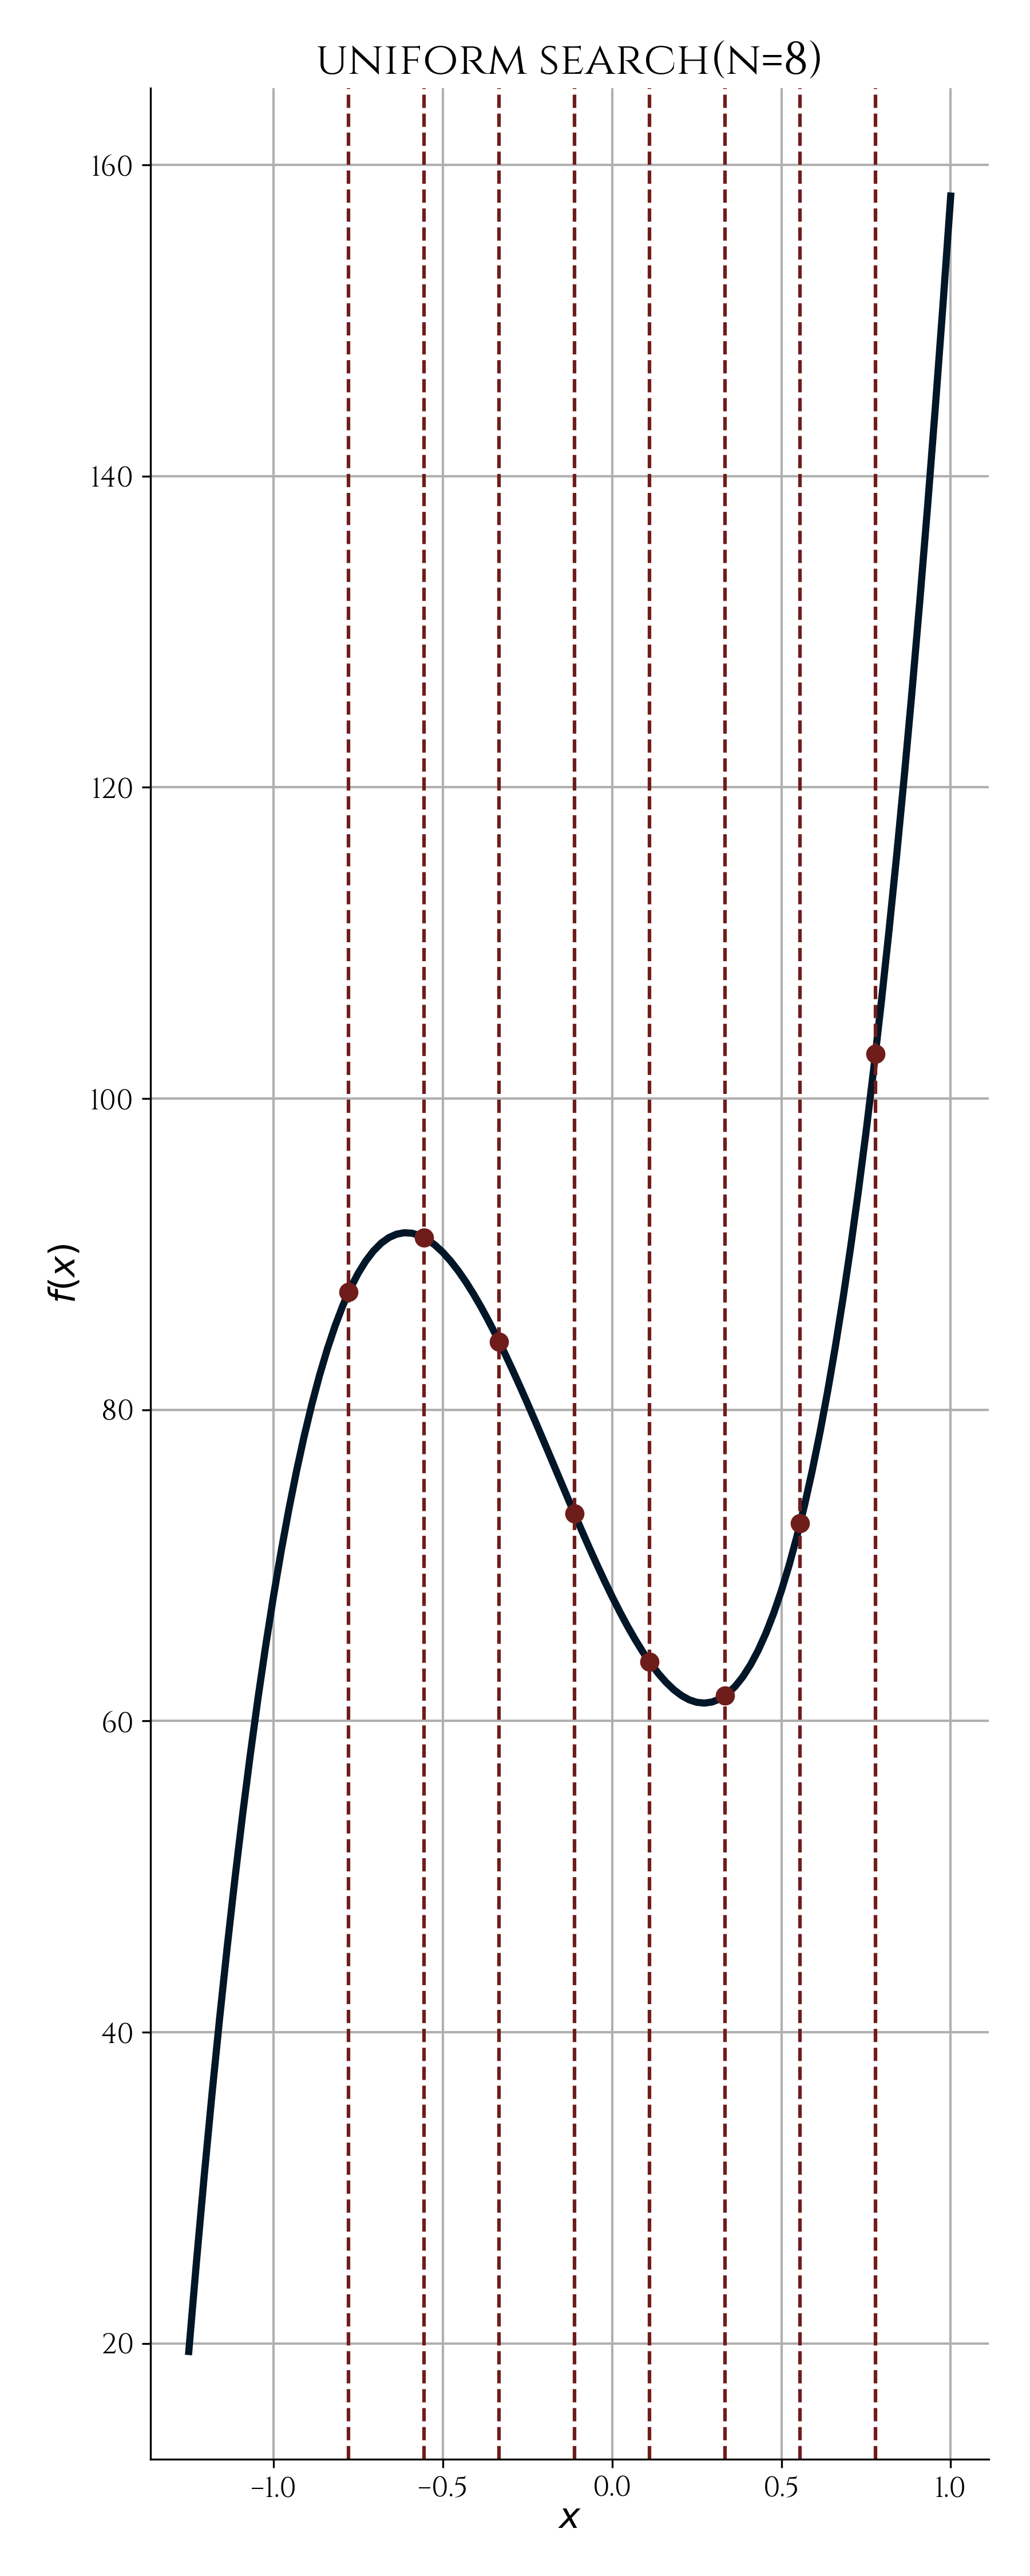
\includegraphics[width=\linewidth]{uniform_search_f_plot(n=8)}
\end{minipage}
\hfill
\begin{minipage}{0.55\textwidth}
    В результате получим график и искомый минимум: 
    \begin{center}
        Minimum found at: (x=0.333333; y=61.629630)
    \end{center}

    Что не сильно отличается от минимумов, найденных \guillemotleft на глаз\guillemotright {} 
    и вручную.
\end{minipage}

Теперь же запустим данный метод на $n=1000$ (в дальнейшем для всех 
методов будет использоваться это значение, если не указано иное) 
и засечем время его исполнения:

\begin{center}
    \begin{lstlisting}[language=Python]
min_point, elapsed_time = optimizer.uniform_search(*INTERVAL) # n = 1000 (default)
print(f'Minimum found at: {min_point:.6f} (execution time: {elapsed_time:.6f}s)')
    \end{lstlisting}
\end{center}

Получим:

\begin{center}
    Minimum found at: (x=0.271728; y=61.152230) (execution time: 0.000846s)
\end{center}

Как можно заметить, результаты уже сильнее отличаются от найденных ранее.

\subsubsection*{Решение при помощи scipy}\vspace{-20pt}\rule{\linewidth}{0.1mm}
\addcontentsline{toc}{subsubsection}{\protect\numberline{}Решение при помощи scipy}

Теперь наследуем еще один класс, но уже для реализации описываемого 
метода с помощью библиотеки scipy:

\begin{center}
    \begin{lstlisting}[language=Python]
# class for scipy implementations
class OptimizationScipy(Optimization):
    # Метод равномерного поиска
    def uniform_search(self, a: float, 
                             b: float,
                             n: int = 1000,
                             add_to_comparison: bool = True):
        # start timer
        start_time = time.perf_counter()
        
        # get result
        res = sp.optimize.brute(self.func, ranges=[(a, b)], 
                                Ns=n, full_output=True)
        minpoint = Point(*res[0], res[1])

        # end timer
        result_time = time.perf_counter() - start_time
        
        # add data to Comparison class
        if add_to_comparison:
            method = Comparison.Method('uniform_search', 'scipy', 
                                        minpoint, result_time)
            cmpr.add_data(method)

        return [minpoint, result_time]
    \end{lstlisting}
\end{center}

И запустим:

\begin{center}
    \begin{lstlisting}[language=Python]
# create optimizer and find minimum
optimizer = OptimizationScipy(func=myfunc)

min_point, elapsed_time = optimizer.uniform_search(*INTERVAL) # n = 1000 (default)
print(f'Minimum found at: {min_point:.6f} (execution time: {elapsed_time:.6f}s)')
    \end{lstlisting}
\end{center}

Получим:

\begin{center}
    Minimum found at: (x=0.271009; y=61.152168) (execution time: 0.011910s)
\end{center}

Данные не сильно различаются с теми, что были найдены \guillemotleft самописной\guillemotright {} 
программой. Причем наша программа работает даже быстрее из-за того, что scipy также 
высчитывает дополнительную информацию (представление оценочной сетки, значения яфункции 
в каждой точке оценочной сетки).

\subsubsection*{Решение при помощи PyTorch}\vspace{-20pt}\rule{\linewidth}{0.1mm}
\addcontentsline{toc}{subsubsection}{\protect\numberline{}Решение при помощи PyTorch}

Наконец наследуем третий класс для реализации метода на PyTorch:

\begin{center}
    \begin{lstlisting}[language=Python]
# class for PyTorch implementations
class OptimizationPyTorch(Optimization):
    # Метод равномерного поиска
    def uniform_search(self, a: float, 
                             b: float,
                             n: int = 1000,
                             add_to_comparison: bool = True,
                             device='cpu') -> Point:
        # start timer
        start_time = time.perf_counter()

        # one-dimensional grid
        x_tenzor = torch.linspace(start=a, end=b, steps=n, device=device)
        
        # get corresponding values
        y_tenzor = self.func(x_tenzor)

        # find the index of the minimum value
        min_ind = torch.argmin(y_tenzor)

        # construct a point
        minpoint = Point(x_tenzor[min_ind], 
                         y_tenzor[min_ind])

        # end timer
        result_time = time.perf_counter() - start_time

        # add data to Comparison class
        if add_to_comparison:
            method = Comparison.Method('uniform_search', 'pytorch', 
                                        minpoint, result_time, device)
            cmpr.add_data(method)

        return [minpoint, result_time]
    \end{lstlisting}
\end{center}

И запустим:

\begin{center}
    \begin{lstlisting}[language=Python]
# create optimizer and find minimum
optimizer = OptimizationPyTorch(func=myfunc)

# use cpu
min_point, elapsed_time = optimizer.uniform_search(*INTERVAL) # n = 1000 (default)
print(f'(cpu)Minimum found at: {min_point:.6f} (execution time: {elapsed_time:.6f}s)')
    \end{lstlisting}
\end{center}

Получим:

\begin{center}
    (cpu)Minimum found at: (x=0.270270; y=61.152233) (execution time: 0.000442s)
\end{center}

Опять же результат похож на найденные ранее, но при этом работает быстрее.\\

В качестве эксперимента запустим данную реализацию метода при большом значении 
$n = 10^8$. Причем запустим как на процессоре (cpu), так и на видеокарте (gpu):

\begin{center}
    \begin{lstlisting}[language=Python]
""" 
check for n = 1 * 10^8
"""
# use cpu
min_point, elapsed_time = optimizer.uniform_search(*INTERVAL, n=int(1e8), 
                                                   add_to_comparison=False)
print(f'(cpu, n=1e8)Minimum found at: {min_point:.6f} (execution time: {elapsed_time:.6f}s)')

# use gpu
device = 'cuda' if torch.cuda.is_available() else 'cpu'
if device == 'cpu':
    raise Exception('cuda is not available')

min_point, elapsed_time = optimizer.uniform_search(*INTERVAL, device=device, 
                                                   n=int(1e8), 
                                                   add_to_comparison=False)
print(f'({'gpu' if device=='cuda' else device}, n=1e8)Minimum found at: {min_point:.6f} (execution time: {elapsed_time:.6f}s)')
    \end{lstlisting}
\end{center}

Итого имеем:

\begin{center}
    (cpu, n=1e8)Minimum found at: (x=0.270859; y=61.152168) (execution time: 1.456683s)
    (gpu, n=1e8)Minimum found at: (x=0.270858; y=61.152168) (execution time: 0.039908s)
\end{center}

Численно результаты особо не отличаются от предыдущих. Также отметим, что исполнение на 
видеокарте ожидаемо быстрее.

% ------------------------------------------------------------------------------------
% -----------------------------------BROKEN LINES-------------------------------------
% ------------------------------------------------------------------------------------

\subsection*{Метод ломаных}\vspace{-20pt}\rule{\linewidth}{0.1mm}
\addcontentsline{toc}{subsection}{\protect\numberline{}Метод ломаных}
\vspace{-30pt}
\subsubsection*{Теория}\vspace{-20pt}\rule{\linewidth}{0.1mm}
\addcontentsline{toc}{subsubsection}{\protect\numberline{}Теория}

\subsubsection*{Аналитическое решение}\vspace{-20pt}\rule{\linewidth}{0.1mm}
\addcontentsline{toc}{subsubsection}{\protect\numberline{}Аналитическое решение}

\subsubsection*{Реализация метода}\vspace{-20pt}\rule{\linewidth}{0.1mm}
\addcontentsline{toc}{subsubsection}{\protect\numberline{}Реализация метода}

\subsubsection*{Решение при помощи scipy}\vspace{-20pt}\rule{\linewidth}{0.1mm}
\addcontentsline{toc}{subsubsection}{\protect\numberline{}Решение при помощи scipy}

\subsubsection*{Решение при помощи PyTorch}\vspace{-20pt}\rule{\linewidth}{0.1mm}
\addcontentsline{toc}{subsubsection}{\protect\numberline{}Решение при помощи PyTorch}

% ------------------------------------------------------------------------------------
% --------------------------------------SECANT----------------------------------------
% ------------------------------------------------------------------------------------

\subsection*{Метод секущих}\vspace{-20pt}\rule{\linewidth}{0.1mm}
\addcontentsline{toc}{subsection}{\protect\numberline{}Метод секущих}
\vspace{-30pt}
\subsubsection*{Теория}\vspace{-20pt}\rule{\linewidth}{0.1mm}
\addcontentsline{toc}{subsubsection}{\protect\numberline{}Теория}

\subsubsection*{Аналитическое решение}\vspace{-20pt}\rule{\linewidth}{0.1mm}
\addcontentsline{toc}{subsubsection}{\protect\numberline{}Аналитическое решение}

\subsubsection*{Реализация метода}\vspace{-20pt}\rule{\linewidth}{0.1mm}
\addcontentsline{toc}{subsubsection}{\protect\numberline{}Реализация метода}

\subsubsection*{Решение при помощи scipy}\vspace{-20pt}\rule{\linewidth}{0.1mm}
\addcontentsline{toc}{subsubsection}{\protect\numberline{}Решение при помощи scipy}

\subsubsection*{Решение при помощи PyTorch}\vspace{-20pt}\rule{\linewidth}{0.1mm}
\addcontentsline{toc}{subsubsection}{\protect\numberline{}Решение при помощи PyTorch}


% ------------------------------------------------------------------------------------
% --------------------------------------NEWTON----------------------------------------
% ------------------------------------------------------------------------------------

\subsection*{Метод Ньютона}\vspace{-20pt}\rule{\linewidth}{0.1mm}
\addcontentsline{toc}{subsection}{\protect\numberline{}Метод Ньютона}
\vspace{-30pt}
\subsubsection*{Теория}\vspace{-20pt}\rule{\linewidth}{0.1mm}
\addcontentsline{toc}{subsubsection}{\protect\numberline{}Теория}

\subsubsection*{Аналитическое решение}\vspace{-20pt}\rule{\linewidth}{0.1mm}
\addcontentsline{toc}{subsubsection}{\protect\numberline{}Аналитическое решение}

\subsubsection*{Реализация метода}\vspace{-20pt}\rule{\linewidth}{0.1mm}
\addcontentsline{toc}{subsubsection}{\protect\numberline{}Реализация метода}

\subsubsection*{Решение при помощи scipy}\vspace{-20pt}\rule{\linewidth}{0.1mm}
\addcontentsline{toc}{subsubsection}{\protect\numberline{}Решение при помощи scipy}

\subsubsection*{Решение при помощи PyTorch}\vspace{-20pt}\rule{\linewidth}{0.1mm}
\addcontentsline{toc}{subsubsection}{\protect\numberline{}Решение при помощи PyTorch}


\end{document}
